% A deep neural network with 3 hidden layers of varying sizes.

\def\layersep{1.5cm}

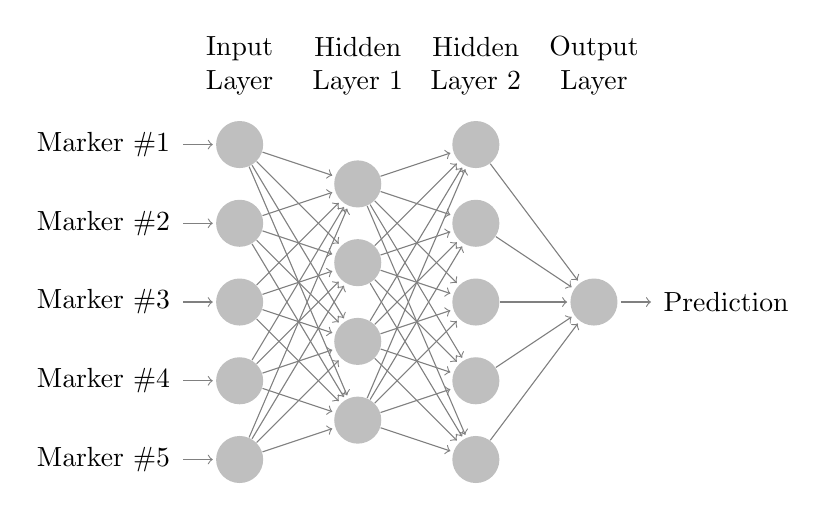
\begin{tikzpicture}[shorten >=1pt, ->, draw=black!50, node distance=\layersep]
    \tikzstyle{every pin edge}=[<-, shorten <=1pt]

    \tikzstyle{neuron}=[circle, fill=black!25,minimum size=17pt, inner sep=0pt]
    \tikzstyle{input neuron}=[neuron];
    \tikzstyle{output neuron}=[neuron];
    \tikzstyle{hidden neuron}=[neuron];

    \tikzstyle{annot}=[text width=4em, text centered]

    \foreach \name / \y in {1,...,5}
        \node[input neuron, pin=left:Marker \#\y] (I-\name) at (0,-\y) {};

    \foreach \name / \y in {1,...,4}
        \path[yshift=-0.5cm]
            node[hidden neuron] (H1-\name) at (\layersep * 1,-\y cm) {};

    \foreach \name / \y in {1,...,5}
        \path[yshift=0.0cm]
            node[hidden neuron] (H2-\name) at (\layersep * 2,-\y cm) {};

    \node[output neuron, pin={[pin edge={->}]right:Prediction}, right of=H2-3] (0) {};

    \foreach \source in {1,...,5}
        \foreach \dest in {1,...,4}
            \path (I-\source) edge (H1-\dest);

    \foreach \source in {1,...,4}
        \foreach \dest in {1,...,5}
            \path (H1-\source) edge (H2-\dest);

    \foreach \source in {1,...,5}
        \path (H2-\source) edge (0);

    \node[annot, above of=I-1, node distance=1cm] (il) {Input Layer};
    \node[annot, right of=il] (hl1) {Hidden Layer 1};
    \node[annot, right of=hl1] (hl2) {Hidden Layer 2};
    \node[annot, right of=hl2] {Output Layer};
\end{tikzpicture}

